\documentclass[11pt]{article}
\usepackage{icmlko}
\begin{document}

\title{폭을 잰 값으로 바꾸니 결정 하나가 뒤집혔다 --- 그리고 그 하나는 재현이 안 된다}
\author{월드모델 실험실}
\date{노트 367 · 2026년 8월 1일}
\maketitle

\begin{abstract}
노트 366이 미리 등록한 것을 한다 --- 미결정 폭을 고정 $0.010$ 에서
\emph{잰 값}으로 바꾸고, \textbf{바꾸기 전에 이 창의 여덟 실험에 소급
적용해 어떤 결정이 바뀌는지 먼저 적는다.} 새 규칙: $|$판 차$| < 2\times$
짝SD \textbf{그리고} 부호가 $[4/12,\,8/12]$ 안일 때만 미결정이고, 아니면
판이 정한다(방향은 평균이 아니라 \textbf{부호 수}로 --- 처음 쓴 규칙이
여기서 틀렸다. 평균 $+0.0001$ 인데 부호가 2/12 인 실험이 있었다).
결과: 여덟 중 배포가 정하던 것이 \textbf{8개에서 3개로} 줄고,
\textbf{뒤집히는 결정은 하나}다 --- 만화 10\%(노트 362, 안 넣음 $\to$
넣음). 그리고 노트 366의 결정은 \emph{이미} 새 규칙과 같았다(옛 규칙대로면
버렸어야 했는데 안 버렸다) --- 규약이 내가 한 일을 뒤늦게 적는 셈이다.
\textbf{그런데 그 하나도 안 넣는다.} 만화 10\%는 \emph{무작위} 178행이라
어느 178행인지가 정해져 있지 않다 --- 짝 뽑기마다 다른 부분집합을 뽑아
평균을 낸 값이고, 실제로 쓰려면 하나를 골라야 하는데 그 선택에 근거가
없다. \textbf{자료 결정은 재현 가능해야 한다} --- 규약에 넣는다.
\end{abstract}

\section{소급부터 적는다}

\begin{center}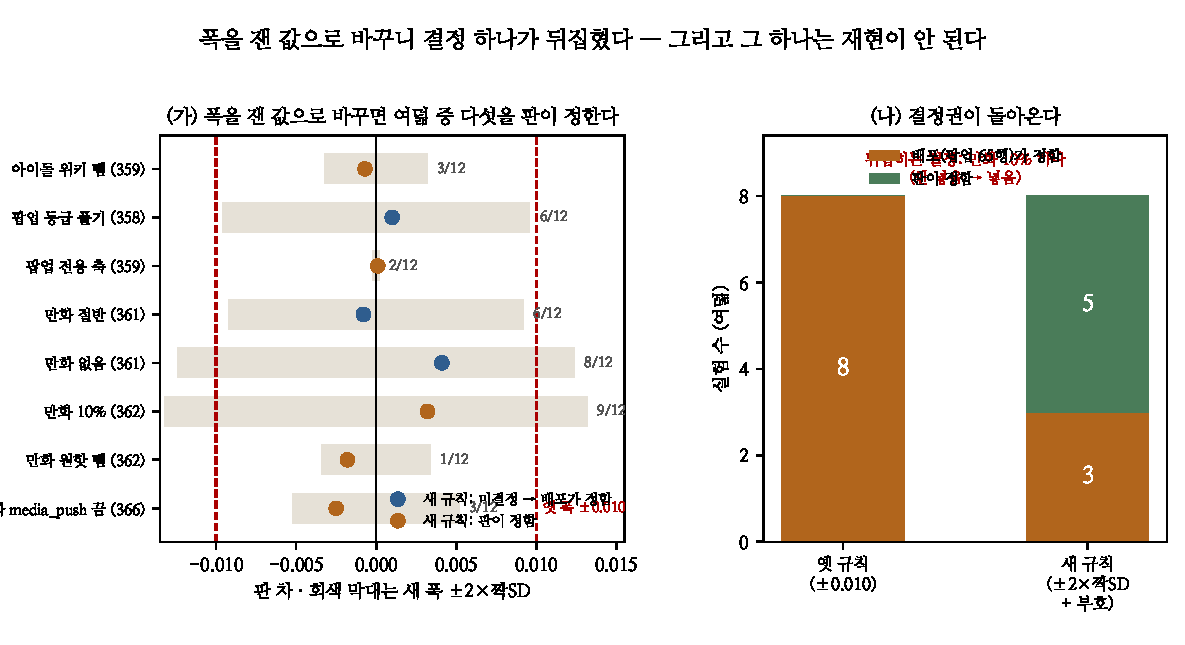
\includegraphics[width=\linewidth]{figs/bandfix.pdf}\end{center}

\begin{center}\small
\begin{tabular}{llrrrrll}
\hline
처치 & 노트 & 판 & $2\!\times\!$SD & 부호 & 팝업 부호 & 옛 & 새 \\
\hline
아이돌 위키 뺌 & 359 & $-0.0007$ & 0.0032 & 3/12 & 4/12 & 배포·안 & 판·안 \\
팝업 등급 풀기 & 358 & $+0.0010$ & 0.0096 & 6/12 & 9/12 & 배포·넣 & 배포·넣 \\
팝업 전용 축 & 359 & $+0.0001$ & 0.0002 & 2/12 & 2/12 & 배포·안 & 판·안 \\
만화 절반 & 361 & $-0.0008$ & 0.0092 & 6/12 & 3/12 & 배포·안 & 배포·안 \\
만화 없음 & 361 & $+0.0041$ & 0.0124 & 8/12 & 2/12 & 배포·안 & 배포·안 \\
\textbf{만화 10\%} & 362 & $+0.0032$ & 0.0132 & \textbf{9/12} & 3/12 & 배포·안 & \textbf{판·넣} \\
만화 원핫 뺌 & 362 & $-0.0018$ & 0.0034 & 1/12 & 6/12 & 배포·안 & 판·안 \\
\texttt{media\_push} 끔 & 366 & $-0.0025$ & 0.0052 & 3/12 & 11/12 & 배포·\textbf{넣} & 판·안 \\
\hline
\end{tabular}
\end{center}

\textbf{배포가 정하던 것이 8개에서 3개로 준다.} 그리고 \textbf{뒤집히는
결정은 만화 10\% 하나}다.

\textbf{노트 366은 이미 새 규칙이었다.} 표의 마지막 줄을 보면 옛 규칙은
``배포 · 넣음''(즉 축을 버려라)이고 나는 안 버렸다. 그때 근거로 쓴 것이
``판 부호가 9/12로 서 있다''였는데, 그것이 정확히 새 규칙의 조항이다.
\textbf{규약이 내가 한 일을 뒤늦게 적는 것이지 새로 시키는 게 아니다} ---
그래서 이 개정은 결과를 보고 규칙을 고른 것이 아니다.

\textbf{방향은 부호 수로 정한다.} 처음 쓴 규칙은 방향을 평균의 부호로
정했는데, ``팝업 전용 축''이 평균 $+0.0001$ 에 부호 \textbf{2/12} 였다 ---
평균은 양수인데 열둘 중 열이 음수다. 노트 359가 이미 ``열둘 중 열이
바이트까지 같다''로 그 실험을 읽었다. \textbf{평균이 아니라 부호를 쓴다.}

\section{그 하나도 안 넣는다 --- 재현}

만화 10\%는 ``만화 학습 1,783행 중 \emph{무작위} 178행만 남긴다''이다.
짝 뽑기 열두 번에서 매번 다른 부분집합을 뽑았고 $+0.0032$(9/12)는 그
평균이다. \textbf{실제로 쓰려면 178행 하나를 골라야 한다.}

\begin{itemize}
\item 어느 178행인지에 근거가 없다. 씨앗을 적어 두면 재현은 되지만
\emph{왜 그 씨앗인가}에는 답이 없다.
\item 다른 씨앗을 고르면 다른 판이 나온다 --- 노트 361이 절반에서
$-0.0008$, 노트 362가 10\%에서 $+0.0032$ 를 얻은 것도 부분집합마다
흔들린 값의 평균이다.
\item \textbf{그리고 더 나은 길이 이미 있다.} 노트 363 · 364가 만화 문제를
회계로 정리했고 노트 365가 258행을 긁어 뒀다. \emph{지우는} 대신
\emph{채점되게} 만들면 같은 자리를 근거 있게 닫는다.
\end{itemize}

\textbf{규약에 넣는다: 자료 결정은 재현 가능해야 한다.} 무작위 부분집합은
측정에는 써도 챔피언에는 안 넣는다. 이것은 폭 규칙과 별개의 조항이고,
그래서 폭을 고치면서도 이 결정은 안 바뀐다.

\section{새 규약}

\begin{quote}
\textbf{미결정}은 $|$판 차$| < 2\times$짝SD \textbf{이고} 부호가
$[4/12,\,8/12]$ 안일 때다. 그때만 배포(팝업)가 정한다. \\
\textbf{아니면 판이 정한다} --- 방향은 부호 수로($\ge 9/12$ 면 넣고
$\le 3/12$ 면 안 넣는다). \\
\textbf{그리고} 어느 도메인도 $|t|>2.77$ 로 안 나빠져야 한다(노트 275 ②는
그대로). \\
\textbf{자료 결정은 재현 가능해야 한다} --- 무작위 부분집합은 측정 전용.
\end{quote}

\textbf{왜 $2\times$짝SD 인가.} 노트 352가 판의 \emph{수준} SD 를 0.0161,
\emph{짝} SD 를 0.0031 로 쟀다. 옛 폭 $0.010$ 은 그 사이 어디도 아니고
노트 245가 옛 판에서 고른 수다. 짝SD 는 실험마다 실제로 재는 값이라
폭이 자료를 따라 움직인다 --- 얇은 실험에서는 넓고 촘촘한 실험에서는
좁다.

\section{남은 것}

\begin{center}
\begin{tabular}{ll}
\hline
갈래 & 지금 아는 것 \\
\hline
\textbf{만화 \texttt{media\_push} 다시 만들기} & 링크 2,041건 받아 뒀다 \\
 & (외부 링크 중앙 3 · 예고편 24.9\%). 옛 값도 같이 \\
 & 다시 만들고 짝으로 잰다. 그러면 258행이 들어간다 \\
팝업 실측 41행 & 노트 360 · 364 · 366. 팝업이 결정권까지 갖고 있다 \\
세계애니 fill 도 자리 기준 & 노트 365. 같은 덫이 하나 더 \\
\hline
\end{tabular}
\end{center}

첫 줄이 이제 막힌 데가 없다 --- 재료가 있고, 무엇을 재야 하는지도 정해졌다.

\end{document}
